\documentclass[12pt,a4paper]{article}

\usepackage[a4paper,text={16.5cm,25.2cm},centering]{geometry}
\usepackage{lmodern}
\usepackage{amssymb,amsmath}
\usepackage{bm}
\usepackage{graphicx}
\usepackage{microtype}
\usepackage{hyperref}
\setlength{\parindent}{0pt}
\setlength{\parskip}{1.2ex}

\hypersetup
       {   pdfauthor = { Gilberto Boaretto & Daniel Coutinho },
           pdftitle={ Hansen's model },
           colorlinks=TRUE,
           linkcolor=black,
           citecolor=blue,
           urlcolor=blue
       }

\title{ Hansen's model }

\author{ Gilberto Boaretto & Daniel Coutinho }

\date{ December, 2019 }

\usepackage{upquote}
\usepackage{listings}
\usepackage{xcolor}
\lstset{
    basicstyle=\ttfamily\footnotesize,
    upquote=true,
    breaklines=true,
    breakindent=0pt,
    keepspaces=true,
    showspaces=false,
    columns=fullflexible,
    showtabs=false,
    showstringspaces=false,
    escapeinside={(*@}{@*)},
    extendedchars=true,
}
\newcommand{\HLJLt}[1]{#1}
\newcommand{\HLJLw}[1]{#1}
\newcommand{\HLJLe}[1]{#1}
\newcommand{\HLJLeB}[1]{#1}
\newcommand{\HLJLo}[1]{#1}
\newcommand{\HLJLk}[1]{\textcolor[RGB]{148,91,176}{\textbf{#1}}}
\newcommand{\HLJLkc}[1]{\textcolor[RGB]{59,151,46}{\textit{#1}}}
\newcommand{\HLJLkd}[1]{\textcolor[RGB]{214,102,97}{\textit{#1}}}
\newcommand{\HLJLkn}[1]{\textcolor[RGB]{148,91,176}{\textbf{#1}}}
\newcommand{\HLJLkp}[1]{\textcolor[RGB]{148,91,176}{\textbf{#1}}}
\newcommand{\HLJLkr}[1]{\textcolor[RGB]{148,91,176}{\textbf{#1}}}
\newcommand{\HLJLkt}[1]{\textcolor[RGB]{148,91,176}{\textbf{#1}}}
\newcommand{\HLJLn}[1]{#1}
\newcommand{\HLJLna}[1]{#1}
\newcommand{\HLJLnb}[1]{#1}
\newcommand{\HLJLnbp}[1]{#1}
\newcommand{\HLJLnc}[1]{#1}
\newcommand{\HLJLncB}[1]{#1}
\newcommand{\HLJLnd}[1]{\textcolor[RGB]{214,102,97}{#1}}
\newcommand{\HLJLne}[1]{#1}
\newcommand{\HLJLneB}[1]{#1}
\newcommand{\HLJLnf}[1]{\textcolor[RGB]{66,102,213}{#1}}
\newcommand{\HLJLnfm}[1]{\textcolor[RGB]{66,102,213}{#1}}
\newcommand{\HLJLnp}[1]{#1}
\newcommand{\HLJLnl}[1]{#1}
\newcommand{\HLJLnn}[1]{#1}
\newcommand{\HLJLno}[1]{#1}
\newcommand{\HLJLnt}[1]{#1}
\newcommand{\HLJLnv}[1]{#1}
\newcommand{\HLJLnvc}[1]{#1}
\newcommand{\HLJLnvg}[1]{#1}
\newcommand{\HLJLnvi}[1]{#1}
\newcommand{\HLJLnvm}[1]{#1}
\newcommand{\HLJLl}[1]{#1}
\newcommand{\HLJLld}[1]{\textcolor[RGB]{148,91,176}{\textit{#1}}}
\newcommand{\HLJLs}[1]{\textcolor[RGB]{201,61,57}{#1}}
\newcommand{\HLJLsa}[1]{\textcolor[RGB]{201,61,57}{#1}}
\newcommand{\HLJLsb}[1]{\textcolor[RGB]{201,61,57}{#1}}
\newcommand{\HLJLsc}[1]{\textcolor[RGB]{201,61,57}{#1}}
\newcommand{\HLJLsd}[1]{\textcolor[RGB]{201,61,57}{#1}}
\newcommand{\HLJLsdB}[1]{\textcolor[RGB]{201,61,57}{#1}}
\newcommand{\HLJLsdC}[1]{\textcolor[RGB]{201,61,57}{#1}}
\newcommand{\HLJLse}[1]{\textcolor[RGB]{59,151,46}{#1}}
\newcommand{\HLJLsh}[1]{\textcolor[RGB]{201,61,57}{#1}}
\newcommand{\HLJLsi}[1]{#1}
\newcommand{\HLJLso}[1]{\textcolor[RGB]{201,61,57}{#1}}
\newcommand{\HLJLsr}[1]{\textcolor[RGB]{201,61,57}{#1}}
\newcommand{\HLJLss}[1]{\textcolor[RGB]{201,61,57}{#1}}
\newcommand{\HLJLssB}[1]{\textcolor[RGB]{201,61,57}{#1}}
\newcommand{\HLJLnB}[1]{\textcolor[RGB]{59,151,46}{#1}}
\newcommand{\HLJLnbB}[1]{\textcolor[RGB]{59,151,46}{#1}}
\newcommand{\HLJLnfB}[1]{\textcolor[RGB]{59,151,46}{#1}}
\newcommand{\HLJLnh}[1]{\textcolor[RGB]{59,151,46}{#1}}
\newcommand{\HLJLni}[1]{\textcolor[RGB]{59,151,46}{#1}}
\newcommand{\HLJLnil}[1]{\textcolor[RGB]{59,151,46}{#1}}
\newcommand{\HLJLnoB}[1]{\textcolor[RGB]{59,151,46}{#1}}
\newcommand{\HLJLoB}[1]{\textcolor[RGB]{102,102,102}{\textbf{#1}}}
\newcommand{\HLJLow}[1]{\textcolor[RGB]{102,102,102}{\textbf{#1}}}
\newcommand{\HLJLp}[1]{#1}
\newcommand{\HLJLc}[1]{\textcolor[RGB]{153,153,119}{\textit{#1}}}
\newcommand{\HLJLch}[1]{\textcolor[RGB]{153,153,119}{\textit{#1}}}
\newcommand{\HLJLcm}[1]{\textcolor[RGB]{153,153,119}{\textit{#1}}}
\newcommand{\HLJLcp}[1]{\textcolor[RGB]{153,153,119}{\textit{#1}}}
\newcommand{\HLJLcpB}[1]{\textcolor[RGB]{153,153,119}{\textit{#1}}}
\newcommand{\HLJLcs}[1]{\textcolor[RGB]{153,153,119}{\textit{#1}}}
\newcommand{\HLJLcsB}[1]{\textcolor[RGB]{153,153,119}{\textit{#1}}}
\newcommand{\HLJLg}[1]{#1}
\newcommand{\HLJLgd}[1]{#1}
\newcommand{\HLJLge}[1]{#1}
\newcommand{\HLJLgeB}[1]{#1}
\newcommand{\HLJLgh}[1]{#1}
\newcommand{\HLJLgi}[1]{#1}
\newcommand{\HLJLgo}[1]{#1}
\newcommand{\HLJLgp}[1]{#1}
\newcommand{\HLJLgs}[1]{#1}
\newcommand{\HLJLgsB}[1]{#1}
\newcommand{\HLJLgt}[1]{#1}


\begin{document}

\maketitle


\begin{lstlisting}
(*@\HLJLnf{include}@*)(*@\HLJLp{(}@*)(*@\HLJLnf{string}@*)(*@\HLJLp{(}@*)(*@\HLJLnf{pwd}@*)(*@\HLJLp{(),}@*)(*@\HLJLs{"{}/src/gensys.jl"{}}@*)(*@\HLJLp{))}@*)

(*@\HLJLn{theta}@*) (*@\HLJLoB{=}@*) (*@\HLJLnfB{0.36}@*)
(*@\HLJLn{delta}@*) (*@\HLJLoB{=}@*) (*@\HLJLnfB{0.025}@*)
(*@\HLJLn{beta}@*) (*@\HLJLoB{=}@*) (*@\HLJLnfB{0.99}@*)
(*@\HLJLn{A}@*) (*@\HLJLoB{=}@*) (*@\HLJLnfB{1.72}@*)
(*@\HLJLn{h0}@*) (*@\HLJLoB{=}@*) (*@\HLJLnfB{0.58}@*)
(*@\HLJLn{gamma}@*) (*@\HLJLoB{=}@*) (*@\HLJLnfB{0.95}@*)
(*@\HLJLn{sig}@*) (*@\HLJLoB{=}@*) (*@\HLJLnfB{0.0712}@*)

(*@\HLJLn{B}@*) (*@\HLJLoB{=}@*) (*@\HLJLn{A}@*)(*@\HLJLoB{*}@*)(*@\HLJLnf{log}@*)(*@\HLJLp{(}@*)(*@\HLJLni{1}@*)(*@\HLJLoB{-}@*)(*@\HLJLn{h0}@*)(*@\HLJLp{)}@*)(*@\HLJLoB{/}@*)(*@\HLJLn{h0}@*)

(*@\HLJLn{r{\_}bar}@*) (*@\HLJLoB{=}@*) (*@\HLJLni{1}@*)(*@\HLJLoB{/}@*)(*@\HLJLn{beta}@*)(*@\HLJLoB{-}@*)(*@\HLJLp{(}@*)(*@\HLJLni{1}@*)(*@\HLJLoB{-}@*)(*@\HLJLn{delta}@*)(*@\HLJLp{)}@*)

(*@\HLJLn{G0}@*) (*@\HLJLoB{=}@*) (*@\HLJLnf{zeros}@*)(*@\HLJLp{(}@*)(*@\HLJLni{7}@*)(*@\HLJLp{,}@*)(*@\HLJLni{7}@*)(*@\HLJLp{)}@*)
(*@\HLJLn{G1}@*) (*@\HLJLoB{=}@*) (*@\HLJLnf{zeros}@*)(*@\HLJLp{(}@*)(*@\HLJLni{7}@*)(*@\HLJLp{,}@*)(*@\HLJLni{7}@*)(*@\HLJLp{)}@*)
(*@\HLJLn{Pi}@*) (*@\HLJLoB{=}@*) (*@\HLJLnf{zeros}@*)(*@\HLJLp{(}@*)(*@\HLJLni{7}@*)(*@\HLJLp{,}@*)(*@\HLJLni{2}@*)(*@\HLJLp{)}@*)
(*@\HLJLn{Psi}@*) (*@\HLJLoB{=}@*) (*@\HLJLnf{zeros}@*)(*@\HLJLp{(}@*)(*@\HLJLni{7}@*)(*@\HLJLp{)}@*)

(*@\HLJLn{G0}@*)(*@\HLJLp{[}@*)(*@\HLJLni{1}@*)(*@\HLJLp{,}@*)(*@\HLJLni{1}@*)(*@\HLJLp{]}@*) (*@\HLJLoB{=}@*) (*@\HLJLni{1}@*)
(*@\HLJLn{G0}@*)(*@\HLJLp{[}@*)(*@\HLJLni{1}@*)(*@\HLJLp{,}@*)(*@\HLJLni{2}@*)(*@\HLJLp{]}@*) (*@\HLJLoB{=}@*) (*@\HLJLoB{-}@*)(*@\HLJLn{r{\_}bar}@*)(*@\HLJLoB{*}@*)(*@\HLJLn{beta}@*)

(*@\HLJLn{G0}@*)(*@\HLJLp{[}@*)(*@\HLJLni{3}@*)(*@\HLJLp{,}@*)(*@\HLJLni{5}@*)(*@\HLJLp{]}@*) (*@\HLJLoB{=}@*) (*@\HLJLni{1}@*)

(*@\HLJLn{G0}@*)(*@\HLJLp{[}@*)(*@\HLJLni{7}@*)(*@\HLJLp{,}@*)(*@\HLJLni{7}@*)(*@\HLJLp{]}@*) (*@\HLJLoB{=}@*) (*@\HLJLni{1}@*)

(*@\HLJLcs{{\#}{\#}{\#}G1{\#}{\#}{\#}{\#}}@*)

(*@\HLJLn{G1}@*)(*@\HLJLp{[}@*)(*@\HLJLni{1}@*)(*@\HLJLp{,}@*)(*@\HLJLni{1}@*)(*@\HLJLp{]}@*) (*@\HLJLoB{=}@*) (*@\HLJLni{1}@*)

(*@\HLJLn{G1}@*)(*@\HLJLp{[}@*)(*@\HLJLni{2}@*)(*@\HLJLp{,}@*)(*@\HLJLni{1}@*)(*@\HLJLp{]}@*) (*@\HLJLoB{=}@*) (*@\HLJLni{1}@*)
(*@\HLJLn{G1}@*)(*@\HLJLp{[}@*)(*@\HLJLni{2}@*)(*@\HLJLp{,}@*)(*@\HLJLni{3}@*)(*@\HLJLp{]}@*) (*@\HLJLoB{=}@*) (*@\HLJLni{1}@*)
(*@\HLJLn{G1}@*)(*@\HLJLp{[}@*)(*@\HLJLni{2}@*)(*@\HLJLp{,}@*)(*@\HLJLni{4}@*)(*@\HLJLp{]}@*) (*@\HLJLoB{=}@*) (*@\HLJLoB{-}@*)(*@\HLJLni{1}@*)

(*@\HLJLn{G1}@*)(*@\HLJLp{[}@*)(*@\HLJLni{3}@*)(*@\HLJLp{,}@*)(*@\HLJLni{1}@*)(*@\HLJLp{]}@*) (*@\HLJLoB{=}@*) (*@\HLJLoB{-}@*)(*@\HLJLp{(}@*)(*@\HLJLn{r{\_}bar}@*)(*@\HLJLoB{/}@*)(*@\HLJLn{theta}@*)(*@\HLJLoB{-}@*)(*@\HLJLn{delta}@*)(*@\HLJLp{)}@*)
(*@\HLJLn{G1}@*)(*@\HLJLp{[}@*)(*@\HLJLni{3}@*)(*@\HLJLp{,}@*)(*@\HLJLni{4}@*)(*@\HLJLp{]}@*) (*@\HLJLoB{=}@*) (*@\HLJLn{r{\_}bar}@*)(*@\HLJLoB{/}@*)(*@\HLJLn{theta}@*)
(*@\HLJLn{G1}@*)(*@\HLJLp{[}@*)(*@\HLJLni{3}@*)(*@\HLJLp{,}@*)(*@\HLJLni{5}@*)(*@\HLJLp{]}@*) (*@\HLJLoB{=}@*) (*@\HLJLp{(}@*)(*@\HLJLni{1}@*)(*@\HLJLoB{-}@*)(*@\HLJLn{delta}@*)(*@\HLJLp{)}@*)

(*@\HLJLn{G1}@*)(*@\HLJLp{[}@*)(*@\HLJLni{4}@*)(*@\HLJLp{,}@*)(*@\HLJLni{3}@*)(*@\HLJLp{]}@*) (*@\HLJLoB{=}@*) (*@\HLJLni{1}@*)(*@\HLJLoB{-}@*)(*@\HLJLn{theta}@*)
(*@\HLJLn{G1}@*)(*@\HLJLp{[}@*)(*@\HLJLni{4}@*)(*@\HLJLp{,}@*)(*@\HLJLni{4}@*)(*@\HLJLp{]}@*) (*@\HLJLoB{=}@*) (*@\HLJLoB{-}@*)(*@\HLJLni{1}@*)
(*@\HLJLn{G1}@*)(*@\HLJLp{[}@*)(*@\HLJLni{4}@*)(*@\HLJLp{,}@*)(*@\HLJLni{5}@*)(*@\HLJLp{]}@*) (*@\HLJLoB{=}@*) (*@\HLJLn{theta}@*)
(*@\HLJLn{G1}@*)(*@\HLJLp{[}@*)(*@\HLJLni{4}@*)(*@\HLJLp{,}@*)(*@\HLJLni{7}@*)(*@\HLJLp{]}@*) (*@\HLJLoB{=}@*) (*@\HLJLni{1}@*)

(*@\HLJLn{G1}@*)(*@\HLJLp{[}@*)(*@\HLJLni{5}@*)(*@\HLJLp{,}@*)(*@\HLJLni{2}@*)(*@\HLJLp{]}@*) (*@\HLJLoB{=}@*) (*@\HLJLoB{-}@*)(*@\HLJLni{1}@*)
(*@\HLJLn{G1}@*)(*@\HLJLp{[}@*)(*@\HLJLni{5}@*)(*@\HLJLp{,}@*)(*@\HLJLni{4}@*)(*@\HLJLp{]}@*) (*@\HLJLoB{=}@*) (*@\HLJLni{1}@*)
(*@\HLJLn{G1}@*)(*@\HLJLp{[}@*)(*@\HLJLni{5}@*)(*@\HLJLp{,}@*)(*@\HLJLni{5}@*)(*@\HLJLp{]}@*) (*@\HLJLoB{=}@*) (*@\HLJLoB{-}@*)(*@\HLJLni{1}@*)

(*@\HLJLn{G1}@*)(*@\HLJLp{[}@*)(*@\HLJLni{6}@*)(*@\HLJLp{,}@*)(*@\HLJLni{3}@*)(*@\HLJLp{]}@*) (*@\HLJLoB{=}@*) (*@\HLJLoB{-}@*)(*@\HLJLni{1}@*)
(*@\HLJLn{G1}@*)(*@\HLJLp{[}@*)(*@\HLJLni{6}@*)(*@\HLJLp{,}@*)(*@\HLJLni{4}@*)(*@\HLJLp{]}@*) (*@\HLJLoB{=}@*) (*@\HLJLni{1}@*)
(*@\HLJLn{G1}@*)(*@\HLJLp{[}@*)(*@\HLJLni{6}@*)(*@\HLJLp{,}@*)(*@\HLJLni{6}@*)(*@\HLJLp{]}@*) (*@\HLJLoB{=}@*) (*@\HLJLoB{-}@*)(*@\HLJLni{1}@*)

(*@\HLJLn{G1}@*)(*@\HLJLp{[}@*)(*@\HLJLni{7}@*)(*@\HLJLp{,}@*)(*@\HLJLni{7}@*)(*@\HLJLp{]}@*) (*@\HLJLoB{=}@*) (*@\HLJLn{gamma}@*)

(*@\HLJLn{Pi}@*)(*@\HLJLp{[}@*)(*@\HLJLni{1}@*)(*@\HLJLp{,}@*)(*@\HLJLni{1}@*)(*@\HLJLp{]}@*) (*@\HLJLoB{=}@*) (*@\HLJLni{1}@*)
(*@\HLJLn{Pi}@*)(*@\HLJLp{[}@*)(*@\HLJLni{1}@*)(*@\HLJLp{,}@*)(*@\HLJLni{2}@*)(*@\HLJLp{]}@*) (*@\HLJLoB{=}@*) (*@\HLJLoB{-}@*)(*@\HLJLn{beta}@*)(*@\HLJLoB{*}@*)(*@\HLJLn{r{\_}bar}@*)

(*@\HLJLn{Psi}@*)(*@\HLJLp{[}@*)(*@\HLJLni{7}@*)(*@\HLJLp{]}@*) (*@\HLJLoB{=}@*) (*@\HLJLni{1}@*)

(*@\HLJLn{sol1}@*) (*@\HLJLoB{=}@*) (*@\HLJLnf{gensys}@*)(*@\HLJLp{(}@*)(*@\HLJLn{G0}@*)(*@\HLJLp{,}@*)(*@\HLJLn{G1}@*)(*@\HLJLp{,}@*)(*@\HLJLn{Psi}@*)(*@\HLJLp{,}@*)(*@\HLJLn{Pi}@*)(*@\HLJLp{)}@*)
\end{lstlisting}


We give a shock of the same size McCandless gives to his system:


\begin{lstlisting}
(*@\HLJLn{irf1}@*) (*@\HLJLoB{=}@*) (*@\HLJLnf{irf}@*)(*@\HLJLp{(}@*)(*@\HLJLn{sol1}@*)(*@\HLJLp{,}@*)(*@\HLJLni{100}@*)(*@\HLJLp{,}@*)(*@\HLJLnfB{0.01}@*)(*@\HLJLp{)}@*)
\end{lstlisting}


\begin{lstlisting}
(*@\HLJLk{using}@*) (*@\HLJLn{Plots}@*)

(*@\HLJLnf{plot}@*)(*@\HLJLp{(}@*)(*@\HLJLn{irf1}@*)(*@\HLJLp{[}@*)(*@\HLJLoB{:}@*)(*@\HLJLp{,}@*)(*@\HLJLni{1}@*)(*@\HLJLp{],}@*) (*@\HLJLn{w}@*) (*@\HLJLoB{=}@*) (*@\HLJLni{2}@*)(*@\HLJLp{,}@*) (*@\HLJLn{label}@*) (*@\HLJLoB{=}@*) (*@\HLJLs{"{}C"{}}@*)(*@\HLJLp{)}@*)
(*@\HLJLnf{plot!}@*)(*@\HLJLp{(}@*)(*@\HLJLn{irf1}@*)(*@\HLJLp{[}@*)(*@\HLJLoB{:}@*)(*@\HLJLp{,}@*)(*@\HLJLni{2}@*)(*@\HLJLp{],}@*) (*@\HLJLn{w}@*) (*@\HLJLoB{=}@*) (*@\HLJLni{2}@*)(*@\HLJLp{,}@*) (*@\HLJLn{label}@*) (*@\HLJLoB{=}@*) (*@\HLJLs{"{}r"{}}@*)(*@\HLJLp{)}@*)
(*@\HLJLnf{plot!}@*)(*@\HLJLp{(}@*)(*@\HLJLn{irf1}@*)(*@\HLJLp{[}@*)(*@\HLJLoB{:}@*)(*@\HLJLp{,}@*)(*@\HLJLni{3}@*)(*@\HLJLp{],}@*) (*@\HLJLn{w}@*) (*@\HLJLoB{=}@*) (*@\HLJLni{2}@*)(*@\HLJLp{,}@*) (*@\HLJLn{label}@*) (*@\HLJLoB{=}@*) (*@\HLJLs{"{}h"{}}@*)(*@\HLJLp{)}@*)
(*@\HLJLnf{plot!}@*)(*@\HLJLp{(}@*)(*@\HLJLn{irf1}@*)(*@\HLJLp{[}@*)(*@\HLJLoB{:}@*)(*@\HLJLp{,}@*)(*@\HLJLni{4}@*)(*@\HLJLp{],}@*) (*@\HLJLn{w}@*) (*@\HLJLoB{=}@*) (*@\HLJLni{2}@*)(*@\HLJLp{,}@*) (*@\HLJLn{label}@*) (*@\HLJLoB{=}@*) (*@\HLJLs{"{}y"{}}@*)(*@\HLJLp{)}@*)
(*@\HLJLnf{plot!}@*)(*@\HLJLp{(}@*)(*@\HLJLn{irf1}@*)(*@\HLJLp{[}@*)(*@\HLJLoB{:}@*)(*@\HLJLp{,}@*)(*@\HLJLni{5}@*)(*@\HLJLp{],}@*) (*@\HLJLn{w}@*) (*@\HLJLoB{=}@*) (*@\HLJLni{2}@*)(*@\HLJLp{,}@*) (*@\HLJLn{label}@*) (*@\HLJLoB{=}@*) (*@\HLJLs{"{}k"{}}@*)(*@\HLJLp{)}@*)
(*@\HLJLnf{plot!}@*)(*@\HLJLp{(}@*)(*@\HLJLn{irf1}@*)(*@\HLJLp{[}@*)(*@\HLJLoB{:}@*)(*@\HLJLp{,}@*)(*@\HLJLni{6}@*)(*@\HLJLp{],}@*) (*@\HLJLn{w}@*) (*@\HLJLoB{=}@*) (*@\HLJLni{2}@*)(*@\HLJLp{,}@*) (*@\HLJLn{label}@*) (*@\HLJLoB{=}@*) (*@\HLJLs{"{}w"{}}@*)(*@\HLJLp{,}@*) (*@\HLJLn{line}@*) (*@\HLJLoB{=}@*) (*@\HLJLsc{:dash}@*)(*@\HLJLp{,}@*) (*@\HLJLn{color}@*) (*@\HLJLoB{=}@*) (*@\HLJLs{"{}red"{}}@*)(*@\HLJLp{)}@*)
(*@\HLJLnf{hline!}@*)(*@\HLJLp{([}@*)(*@\HLJLni{0}@*)(*@\HLJLp{],}@*) (*@\HLJLn{color}@*) (*@\HLJLoB{=}@*) (*@\HLJLs{"{}black"{}}@*)(*@\HLJLp{,}@*) (*@\HLJLn{w}@*) (*@\HLJLoB{=}@*) (*@\HLJLni{2}@*)(*@\HLJLp{)}@*)
\end{lstlisting}

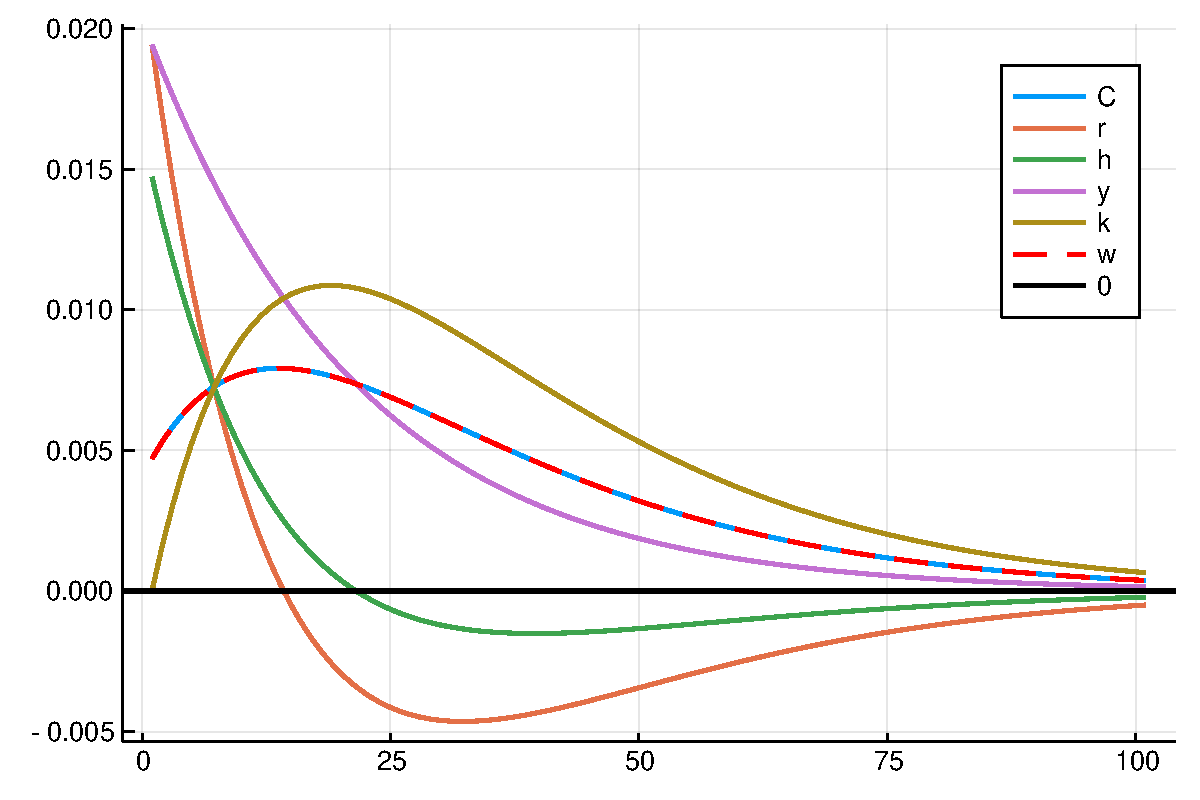
\includegraphics[width=\linewidth]{figures/yvan_3_1.pdf}


\end{document}
